\section{全同粒子}

\begin{quotation}
``我觉得爱因斯坦不完全是愚蠢的。''\qquad 泡利
\end{quotation}

\subsection{全同性原理}


氢原子是最简单的原子, 比氢原子复杂一点的是氦原子, 还有更复杂的原子,
它们的特点是含有多个电子,
即所谓多电子原子。如何处理``多电子''就成了需要研究的问题,
为了简单考虑我们不妨假设多个电子间不存在相互作用, 对每个电子而言,
就回到单电子的问题, 或氢原子的问题,
可以计算出一系列的能级和波函数等等。

我们用$\psi_n(q_1)$表示第一个电子的波函数,
那么在形式上第二个电子的波函数就是$\psi_{n'}(q_2)$,
等等。宗量$q_i$表示第$i$个电子的位置$ \vec{r}_i$和自旋$s_i^z$等,
由于每个电子都处在相同的势场中,
所以对每个电子而言解出来的波函数$\psi_n$在形式上是相同的。
那么所有这些波函数的直接乘积(direct product), 或张量积(tensor
product)$\psi_{n_1}(q_1) \cdot \psi_{n_2}(q_2)
...$就构成了可能的多电子原子的波函数\footnote{由于电子的质量远小于原子核的质量,
对多电子原子而言, 我们研究的其实就是一个多电子的系统,
波函数就是包含多个电子的波函数,
即玻恩-奥本海默近似。}。但是除此之外还需满足一个要求,
即``全同性原理''。

\index{Identical principle: 全同原理}

当我们讲到电子甲和电子乙的时候,
它们是一样的吗?这涉及到我们对两个电子的区分的问题, 如果是经典物理,
这在原则上总是可以做到的, 即对给定物理系统,
我们总可以区分电子甲和电子乙。因为在经典物理学中, 只要给定物理系统,
给定系统内每个粒子的初始位置和动量,
我们总可无限精确地求解出每个粒子的轨迹,
我们可通过追踪这些轨迹来区分任意两个电子。


但这一条在量子力学中是不存在的,
简单说由于不确定原理——如果无限精确地确定了粒子的位置,
那么粒子的动量就是完全不确定的, 反之亦然。在此意义下,
我们能够得到的最多将是一个满足不确定原理的``模糊''轨迹。这样,
在原则上我们就不能区分两个电子了。翻译成波函数的语言就是,
交换系统内两个粒子的宗量(坐标,自旋等)将不会导致波函数有本质的变化,
比如乘上一个复数因子$\lambda$。

\begin{equation*}
  P_{12} \psi(q_1,q_2) = \psi(q_2,q_1) = \lambda \psi(q_1,q_2)
\end{equation*}


如果再交换一次,那么波函数将会回到原来的形式。

\begin{equation*}
  P_{12} \psi (q_2,q_1) = \lambda^2 \psi(q_1,q_2) = \psi(q_1,q_2)
\end{equation*}


这意味着$ \lambda^2 =1 $,即$ \lambda = \pm
1$。这里给出了对全同粒子波函数的限制: 它们必须是交换对称($ \lambda
= 1 $)的或交换反对称($ \lambda =
-1$)的。这要求我们把直接乘积表示下的波函数对称化或反对称化,
满足交换对称的称之为玻色子,
满足交换反对称的称之为费米子。常见的玻色子是: 光子,
声子等(自旋为整数);常见的费米子是: 电子, 正电子, 质子,
中子等(自旋为半整数)。


对称波函数描写的全同粒子是玻色子,服从玻色-爱因斯坦统计:

\index{Bose-Einstein statistics: 玻色-爱因斯坦统计}

\begin{equation}\label{31-3}
f_{BE} \left( \varepsilon  \right) = \left[ {{\mathop{\rm e}\nolimits} ^{\varepsilon /k_B T}  - 1} \right]^{ - 1}
\end{equation}


反对称波函数描写的全同粒子是费米子,服从费米-狄拉克统计:

\index{Fermi-Dirac statistics: 费米-狄拉克统计}

\begin{equation}\label{31-4}
f_{FD} \left( \varepsilon  \right) = \left[ {{\mathop{\rm e}\nolimits} ^{\varepsilon /k_B T}  + 1} \right]^{ - 1}
\end{equation}

实验以及理论都表明:自旋量子数为整数的粒子是玻色子(如:光子$S=1$),
自旋量子数为半奇数的粒子是费米子(如:电子$S=1/2$)。

对于经典粒子,服从玻尔兹曼-麦克斯韦统计:

\begin{equation}\label{31-5}
f_{BM} \left( \varepsilon  \right) = {\mathop{\rm e}\nolimits} ^{ - \varepsilon /k_B T}
\end{equation}


复合粒子是由若干更``基本''的粒子组成的, 如:$\alpha$粒子($_2^4 He$,
由两个质子和两个中子组成,总自旋为$0$),
两个$\alpha$粒子的波函数表示为:

$\psi \left( {n_1 ,\tilde n_1 ,p_1 ,\tilde p_1 ;n_2 ,\tilde n_2 ,p_2 ,\tilde p_2 } \right) = \psi \left( {n_1 ,n_2 ;\tilde n_1 ,\tilde n_2 ;p_1 ,p_2 ;\tilde p_1 ,\tilde p_2 } \right)$

交换一对$\alpha$粒子,相当于组成$\alpha$粒子的质子和中子都交换坐标,共交换四次,
波函数四次变号,总的结果是不变号。所以$\alpha$粒子是玻色子,服从玻色-爱因斯坦统计。
一般而言,如果复合粒子处在相同的量子态(具有相同形式的波函数),
它们就可被看作是全同粒子,例如:处于基态的两个氢原子。

物质波波长$\lambda  = \frac{h}{p} \sim \frac{h}{{\sqrt {2mE}
}}$,考虑到复合粒子平均动能:$\left\langle E \right\rangle  \sim
{\textstyle{3 \over 2}}k_B T$,$\lambda  \sim \frac{h}{{\left(
{3mk_B T} \right)^{1/2} }}$随着复合粒子中粒子数目的增加, 质量将增大,
物质波波长\footnote{因为是用无规则热运动动能估算的,
因此也叫热波波长。}将逐渐变短,
当物质波波长短于复合粒子间距时($\lambda < d$),
波函数交叠区域将会迅速变小, 以致可以忽略,
这时全同粒子可近似地按经典粒子进行处理。 如果降低温度,
物质波波长将会有增大的趋势, 当温度降低到一定程度时,
物质波波长将可与复合粒子间距比较, 这时量子力学效应不可以忽略,
复合粒子必须被看作是全同粒子。在玻色-爱因斯坦凝聚实验中,
使用的就是复合粒子--碱金属原子。甚至在更加复杂的全同粒子--分子中,
也可以观察到玻色-爱因斯坦凝聚。


\subsection{全同粒子的波函数}


\subsubsection{多费米子系波函数}

多费米子系统的波函数满足交换反对称,比如两个费米子的波函数可写为:

\begin{equation}\label{two-fermions}
   \psi_{m,n}^F (q_1,q_2) =\frac{1}{\sqrt{2}} (
\psi_m(q_1)\psi_n(q_2) - \psi_m(q_2) \psi_n(q_1) )
\end{equation}



改写成行列式的样子:


\begin{equation*}
 \psi _{m,n}^F (q_1 ,q_2 ) = \frac{1}{{\sqrt 2 }}\left|
{\begin{array}{*{20}c}
   {\psi _m (q_1 )} & {\psi _m (q_2 )}  \\
   {\psi _n (q_1 )} & {\psi _n (q_2 )}  \\
\end{array}} \right|
\end{equation*}


如果用语言说的话, 这个波函数表示有两个费米子, 一个处于$m$态,
另一个处于$n$态;但我们无法说正是哪一个费米子(宗量为$q_1$)是处在$m$态的,
而另一个费米子(宗量为$q_2$)是处在$n$态的。如果$m=n$的话,
波函数即为$0$, 此即``泡利不相容原理''。


\index{Pauli exclusion principle: 泡利不相容原理}

对$N$个费米子组成的多粒子系而言, 波函数由类似的行列式给出,
$N$个费米子将分别占据$N$个不同的量子态,
归一化因子为:$\frac{1}{\sqrt{N!}}$(这是因为行列式中有 $N!$项)。
多费米子系任意两个费米子不能处于相同量子态, 否则行列式为$0$(
泡利不相容原理\footnote{关于泡利不相容原理,
请参考:http://rugth30.phys.rug.nl/quantummechanics/idpart.htm})。



\begin{figure}[h]
\begin{center}
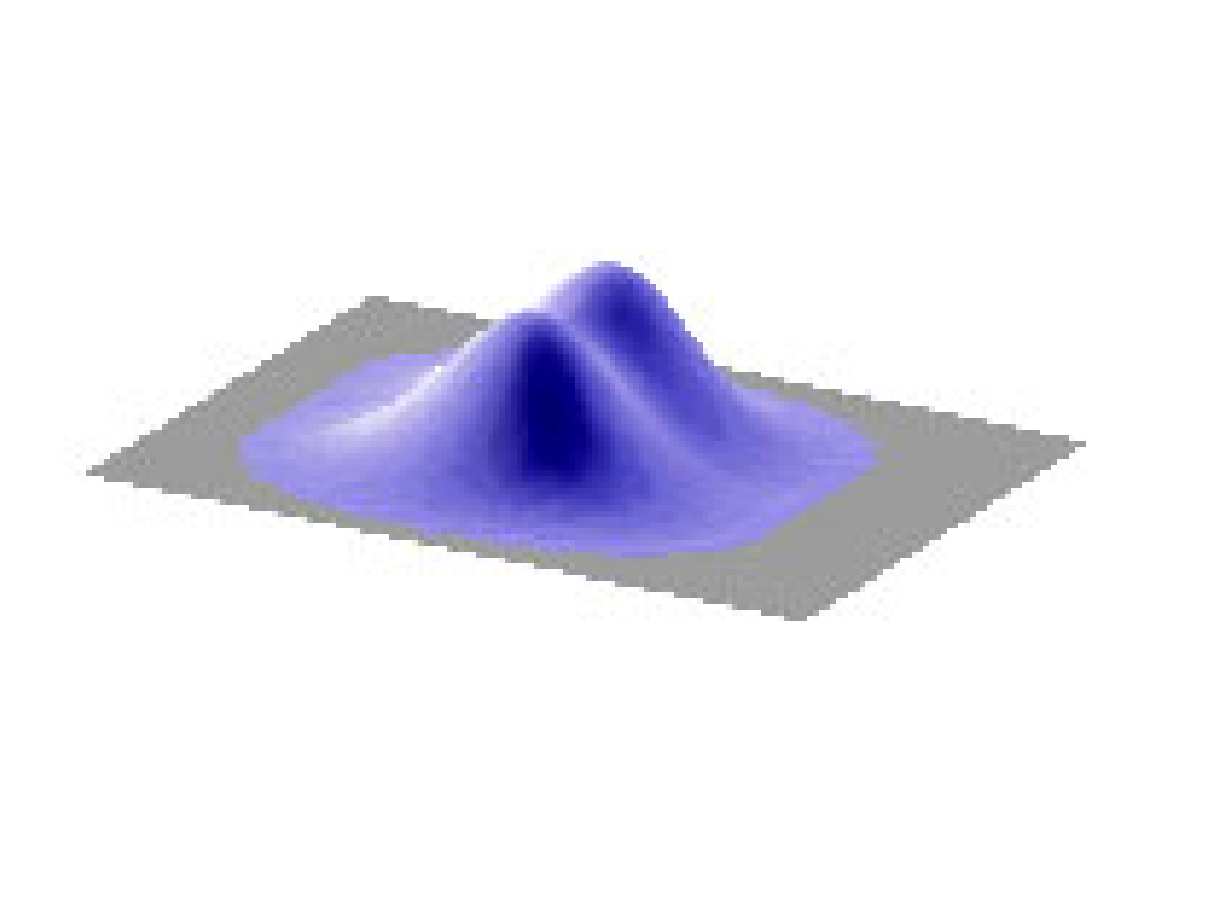
\includegraphics[clip,width=5cm]{IdenticalParticles/31-1.ps}
\caption{全同费米子在空间中的几率分布:不能占据空间中相同点}
\end{center}
\end{figure}


\subsubsection{多玻色子系波函数}

类似地,两个玻色子的波函数可写为:


\begin{equation}\label{two-bosons}
  \psi_{m,n}^B = \frac{1}{\sqrt 2} ( \psi_m(q_1)\psi_n(q_2) +
\psi_m(q_2)\psi_n(q_1))
\end{equation}



由于中间是加号,对玻色子而言无泡利不相容原理,因此$m=n$这样的波函数是允许的。$N$个玻色子组成的多粒子系,其波函数也可形式地写为行列式的样子,但每一项都取“+”号,这样就没有多个全同粒子不许占据相同量子态的限制了,归一化因子为:$\sqrt{\frac{n_1!
n_2 !
...}{N!}}$($\psi_m(q_1)\psi_m(q_2)$和$\psi_m(q_2)\psi_m(q_1)$是一样的,合并相同的项后,
``行列式''中有$\frac{{N!}}{{\mathop \prod \limits_i n_i !}}$),
这里的$n_1$表示有$n_1$个粒子占据第一个量子态。

\index{Bose-Einstein condensate: 玻色-爱因斯坦凝聚}

对于玻色子而言,不存在泡利不相容原理,因此可以有多个玻色子占据相同的量子态,
如果在绝对零度,所有的玻色子将都占据最低能态,这种现象被称为玻色-爱因斯坦凝聚(Bose-Einstein
Condensate)。1995年,美国科罗拉多大学的Wieman小组使用激光冷却技术在$0.000
000 02
K$绝对温度下观察到了${}^{87}Rb$原子的玻色-爱因斯坦凝聚。并因此获得了2001年的诺贝尔物理奖\footnote{关于玻色-爱因斯坦凝聚,
请参考:http://www.colorado.edu/physics/2000/bec/

关于激光冷却与玻色-爱因斯坦凝聚,
请参考:http://online.itp.ucsb.edu/online/plecture/ketterle/}。

玻色-爱因斯坦凝聚即可发生在动量空间、也可发生在实空间。
如发生在实空间,大量玻色子(实验中是碱金属原子)将占据空间相同位置,
这在经典物理学中是不可思异的。



\begin{figure}[h]
\begin{center}
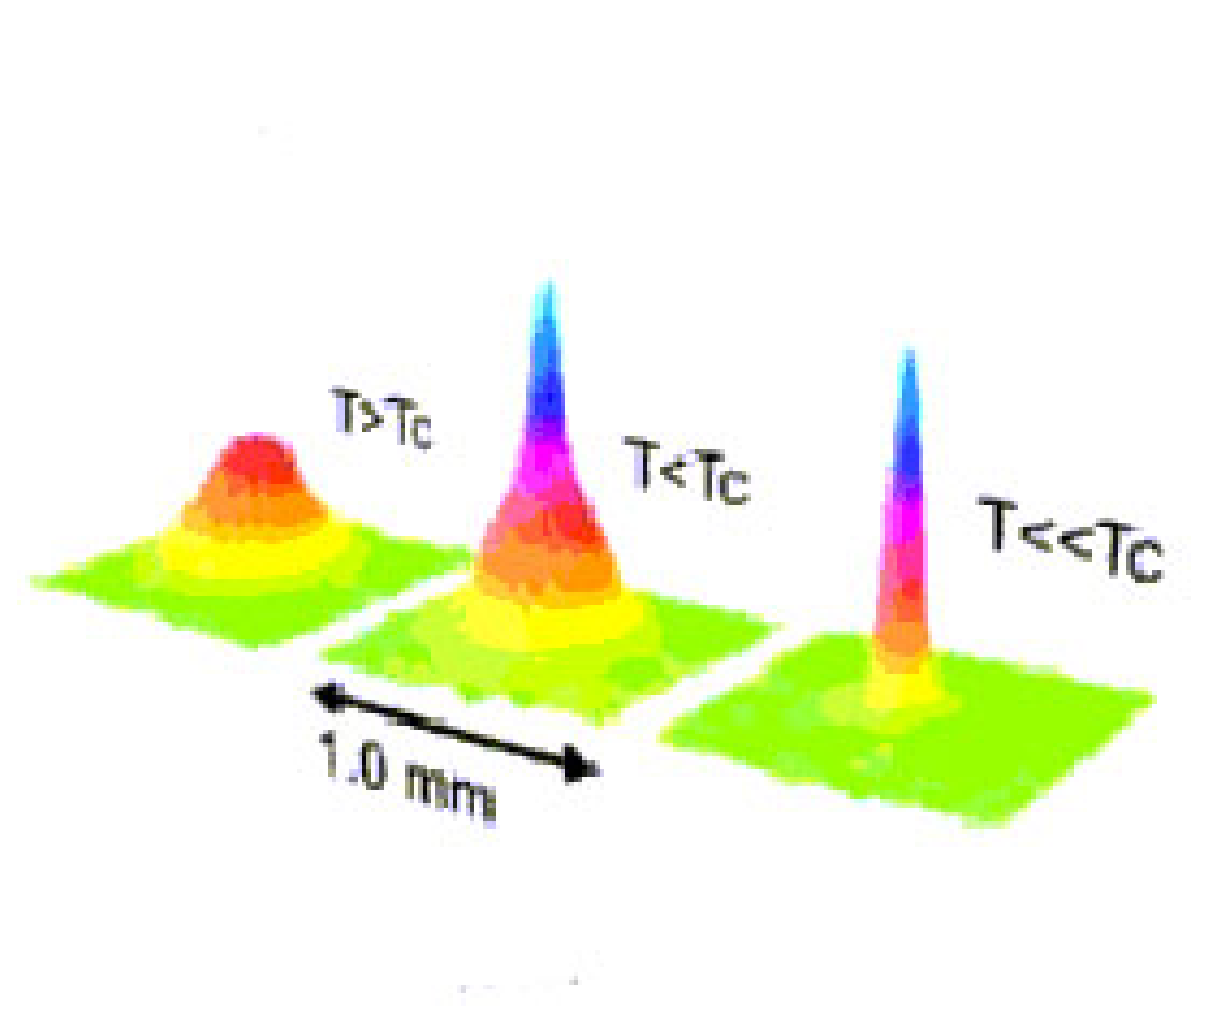
\includegraphics[clip,width=5cm]{IdenticalParticles/31-2.ps}
\caption{纳原子气中实现的玻色-爱因斯坦凝聚}
\end{center}
\end{figure}


\subsubsection{写出多粒子系波函数的步骤}

(1)把物理问题化为无相互作用的多粒子系$H = \sum\limits_{i}{h_i}
$;(2)对单粒子哈密顿$h \psi_n = \epsilon_n
\psi_n$求解量子力学本征值问题;(3)得到多粒子系的直接乘积表示;(4)对多玻色子系统或多费米子系统分别将直接乘积表示对称化或反对称化。



\subsubsection{$N$个全同粒子的归一化波函数}

不考虑粒子间的相互作用,两全同粒子体系的哈密顿:

\begin{equation}\label{31-6}
H = H_0 \left( {q_1 } \right) + H_0 \left( {q_2 } \right)
\end{equation}


对于全同粒子而言,$H_0 \left( {q_1 } \right)$与$H_0 \left( {q_2 }
\right)$形式相同,因此有相同形式的本征函数,本征值分别为$\varepsilon
_1 ,\varepsilon _2 $。


\begin{equation}\label{31-7}
\left\{ \begin{array}{l}
 H_0 \left( {q_1 } \right)\phi _1 \left( {q_1 } \right) = \varepsilon _1 \phi _1 \left( {q_1 } \right) \\
 H_0 \left( {q_2 } \right)\phi _2 \left( {q_2 } \right) = \varepsilon _2 \phi _2 \left( {q_2 } \right) \\
 \end{array} \right.
\end{equation}


总的薛定谔方程:$H\phi \left( {q_1 ,q_2 } \right) = E\phi \left(
{q_1 ,q_2 } \right)$

由于粒子间无相互作用,可以分离变量求解:

$\phi \left( {q_1 ,q_2 } \right) = \phi _1 \left( {q_1 } \right)\phi
_2 \left( {q_2 } \right)$, $E = \varepsilon _1  + \varepsilon _2 $

如果粒子1处于$\phi _2 $状态,粒子2处于$\phi _1 $状态:

$\phi \left( {q_2 ,q_1 } \right) = \phi _2 \left( {q_1 } \right)\phi
_1 \left( {q_2 } \right) = \phi _1 \left( {q_2 } \right)\phi _2
\left( {q_1 } \right)$, $E = \varepsilon _2  + \varepsilon _1  =
\varepsilon _1  + \varepsilon _2 $(交换简并)


根据全同粒子性质,全同粒子波函数必须是对称或反对称的。




\begin{description}
    \item[费米子]

\begin{equation}\label{31-8}
\phi _A \left( {q_1 ,q_2 ,...,q_N } \right) = \frac{1}{{\sqrt {N!}
}}\left| {\begin{array}{*{20}c}
   {\phi _1 \left( {q_1 } \right)} & {\phi _1 \left( {q_2 } \right)} & {...} & {\phi _1 \left( {q_N } \right)}  \\
   {\phi _2 \left( {q_1 } \right)} & {\phi _2 \left( {q_2 } \right)} & {...} & {\phi _2 \left( {q_N } \right)}  \\
   {...} & {...} & {...} & {...}  \\
   {\phi _N \left( {q_1 } \right)} & {\phi _N \left( {q_2 } \right)} & {...} & {\phi _N \left( {q_N } \right)}  \\
\end{array}} \right|
\end{equation}

满足:$\phi _A \left( {q_1 ,q_2 ,...,q_N } \right) =  - \phi _A
\left( {q_2 ,q_1 ,...,q_N } \right)$;
如果存在两个或两个以上相同的量子态$\varepsilon _1  = \varepsilon _2
$:$\phi _A \left( {q_1 ,q_2 ,...,q_N } \right) =
0$,(即:泡利原理)。


    \item[玻色子]

可以存在相同的量子态,假设$n_i$个粒子处在$\varepsilon _i $态,则:$N
= \sum {n_i } $,$E = \sum {n_i \varepsilon _i } $

\begin{equation}\label{31-9}
\phi _S \left( {q_1 ,q_2 ,...,q_N } \right) = \sqrt
{\frac{{\prod\limits_i {n_i !} }}{{N!}}} \sum\limits_P {P\left[
{\phi _{\varepsilon _1 } \left( {q_1 } \right)\phi _{\varepsilon _2
} \left( {q_2 } \right)...\phi _{\varepsilon _N } \left( {q_N }
\right)} \right]}
\end{equation}

P表示对粒子坐标$\left\{ {\varepsilon _i }
\right\}$进行轮换\footnote{参考曾谨言《量子力学 卷I》第291页}。

\end{description}


\subsection{玻色-爱因斯坦凝聚发生温度计算}


\begin{figure}[h]
\begin{center}
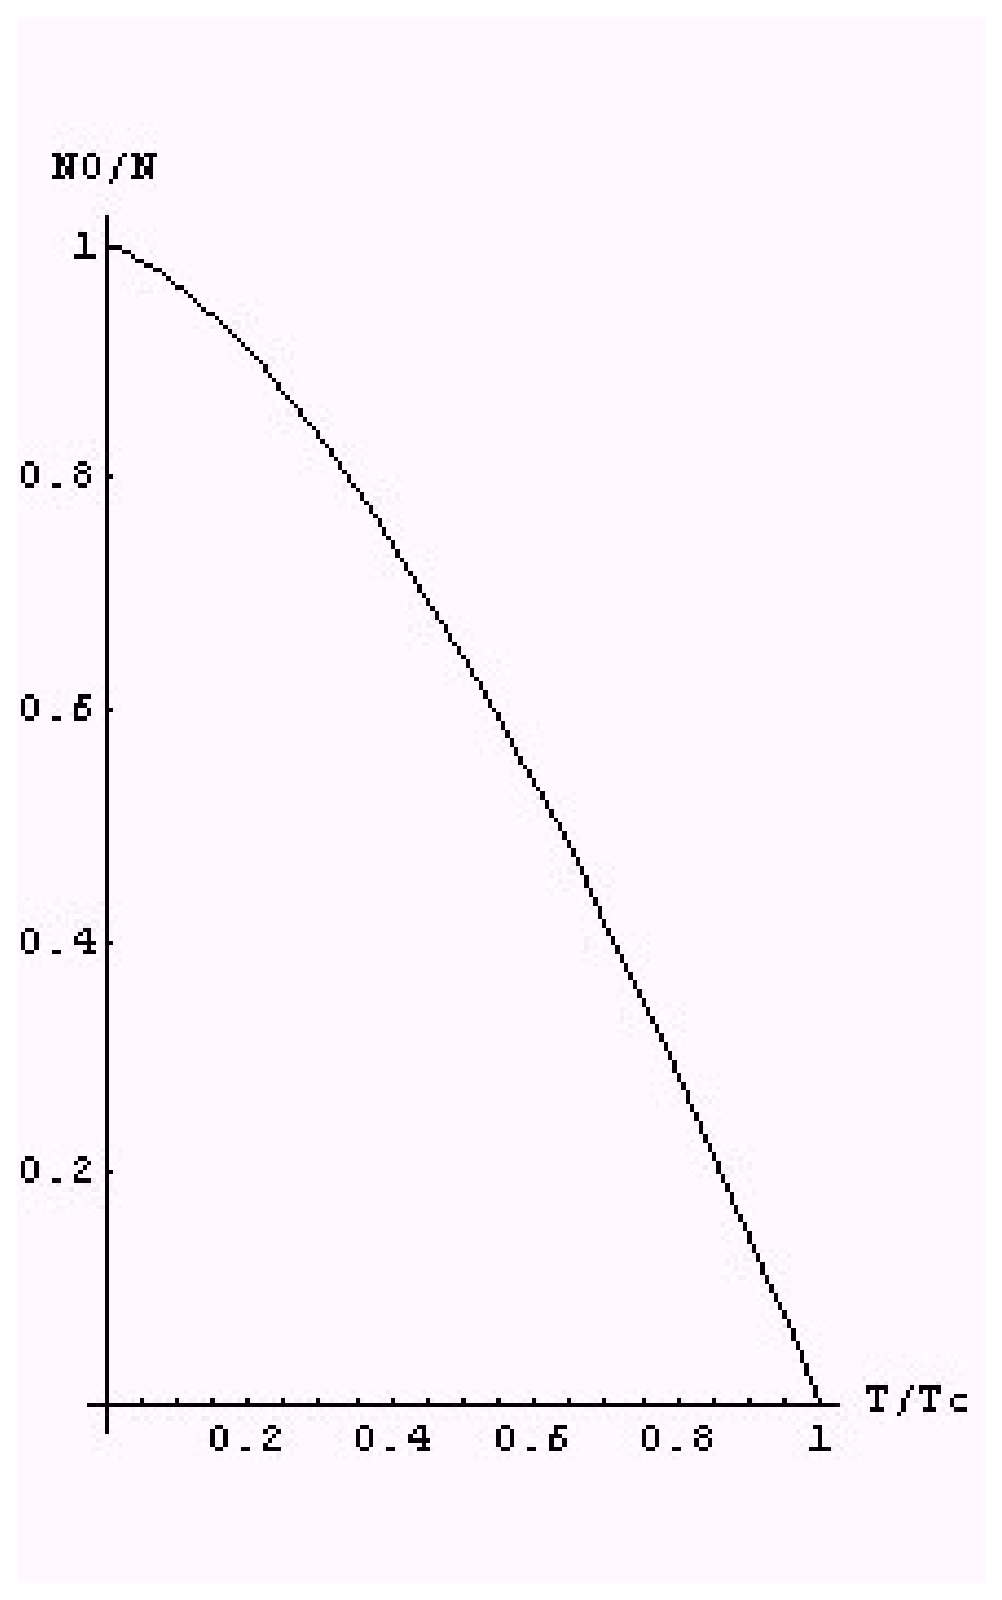
\includegraphics[clip,width=5cm]{IdenticalParticles/31-3.ps}
\caption{发生玻色-爱因斯坦凝聚的粒子百分比$N_0 / N$随温度$T_c /
T$变化的关系(理论曲线)}
\end{center}
\end{figure}


1995年,Ketterle(Ketterle也获得了2001年诺贝尔物理奖)使用Na原子为玻色子,
在实验中观测到了Na原子的玻色-爱因斯坦凝聚。实验中Na原子气的数密度为:$n \sim 1.5 \times 10^{20} m^{ - 3} $,在$T_c  \approx \left( {2 \pm 0.5} \right) \times 10^{ - 6} K$开始观察到玻色-爱因斯坦凝聚。我们现在来求玻色-爱因斯坦凝聚发生温度的理论公式\footnote{参考:K.B. Davis, et al., \emph{Phys. Rev. Lett}. \textbf{75}, 3969 (1995);

黄克逊,《统计力学》;}。

假设有$N$个无相互作用玻色子,在温度$T$时,部分玻色子$N_0$由于玻色-爱因斯坦凝聚占据最低能态$E_0$,其余玻色子$N_e  = N - N_0 $则占据各激发态$E_1 ,E_2 ,...$

$N = N_0  + N_e  = N_0  + \int_0^\infty  {f\left( \varepsilon  \right)D\left( \varepsilon  \right)d\varepsilon } $, $f\left( \varepsilon  \right) = \frac{1}{{\exp \left( {{\textstyle{{\varepsilon  - \mu } \over {k_B T}}}} \right) - 1}}$


$D\left( \varepsilon  \right) = \frac{{dg}}{{d\varepsilon }}$为态密度,$dg = \left( {2s + 1} \right)\frac{{d^3 pd^3 q}}{{h^3 }} = \frac{V}{{h^3 }}4\pi p^2 dp$(假设玻色子自旋为0)

$\varepsilon  = \frac{{p^2 }}{{2\mu }}$, $dp = \frac{{\mu d\varepsilon }}{p}$, 所以态密度为:

\begin{equation}\label{31-1-1}
D\left( \varepsilon  \right) = \frac{{dg}}{{d\varepsilon }} = \frac{V}{{4\pi ^2 }}\left( {\frac{{2\mu }}{{\hbar ^2 }}} \right)^{3/2} \sqrt \varepsilon
\end{equation}


激发态粒子总数:

\begin{equation}\label{31-1-2}
\begin{array}{l}
 N_e  = \int_0^\infty  {f\left( \varepsilon  \right)D\left( \varepsilon  \right)d\varepsilon }  = \int_0^\infty  {\frac{1}{{\exp \left( {{\textstyle{{\varepsilon  - \mu } \over {k_B T}}}} \right) - 1}}\frac{V}{{4\pi ^2 }}\left( {\frac{{2\mu }}{{\hbar ^2 }}} \right)^{3/2} \sqrt \varepsilon  d\varepsilon }  \\
  = \frac{V}{{4\pi ^2 }}\left( {\frac{{2\mu }}{{\hbar ^2 }}} \right)^{3/2} \int_0^\infty  {\frac{1}{{\exp \left( {{\textstyle{{\varepsilon  - \mu } \over {k_B T}}}} \right) - 1}}\sqrt \varepsilon  d\varepsilon }  \\
 \end{array}
\end{equation}

在绝对零度时,全部玻色子发生玻色-爱因斯坦凝聚,重新选择能量零点为系统基态能($\varepsilon  = 0$):

\begin{center}
$\begin{array}{l}
 \mathop {\lim }\limits_{T \to 0} f\left( \varepsilon  \right) = \mathop {\lim }\limits_{T \to 0} \frac{1}{{\exp \left( {{\textstyle{{ - \mu } \over {k_B T}}}} \right) - 1}} = N \Rightarrow \mathop {\lim }\limits_{T \to 0} \exp \left( {{\textstyle{{ - \mu } \over {k_B T}}}} \right) - 1 = \frac{1}{N} \\
 \mathop {\lim }\limits_{T \to 0} \exp \left( {{\textstyle{{ - \mu } \over {k_B T}}}} \right) = 1 + \frac{1}{N} \Rightarrow \mathop {\lim }\limits_{T \to 0} \left( {1 - {\textstyle{\mu  \over {k_B T}}} + ...} \right) = 1 + \frac{1}{N} \\
 \mathop {\lim }\limits_{T \to 0} \left( { - {\textstyle{\mu  \over {k_B T}}}} \right) = \frac{1}{N} \Rightarrow \mathop {\lim }\limits_{T \to 0} \mu  =  - \frac{{k_B T}}{N} \\
 \end{array}$
\end{center}


由于宏观系统$N \to \infty $,所以:$\frac{\mu }{{k_B T}} \to 0$

\begin{equation}\label{31-1-3}
\begin{array}{c}
N_e  = \frac{V}{{4\pi ^2 }}\left( {\frac{{2\mu }}{{\hbar ^2 }}} \right)^{3/2} \int_0^\infty  {\frac{1}{{\exp \left( {{\textstyle{{\varepsilon  - \mu } \over {k_B T}}}} \right) - 1}}\sqrt \varepsilon  d\varepsilon }  \\
\quad = \frac{V}{{4\pi ^2 }}\left( {\frac{{2\mu }}{{\hbar ^2 }}} \right)^{3/2} \int_0^\infty  {\frac{1}{{\exp \left( {{\textstyle{\varepsilon  \over {k_B T}}}} \right) - 1}}\sqrt \varepsilon  d\varepsilon }
\end{array}
\end{equation}

变量变换:$x = \frac{\varepsilon }{{k_B T}}, d\varepsilon  = k_B Tdx$

\begin{equation}\label{31-1-4}
\begin{array}{l}
 N_e  = \frac{V}{{4\pi ^2 }}\left( {\frac{{2\mu k_B T}}{{\hbar ^2 }}} \right)^{3/2} \int_0^\infty  {\frac{1}{{{\mathop{\rm e}\nolimits} ^x  - 1}}\sqrt x dx}  = \frac{V}{{4\pi ^2 }}\left( {\frac{{2\mu k_B T}}{{\hbar ^2 }}} \right)^{3/2} \Gamma \left[ {{\textstyle{3 \over 2}}} \right]\zeta \left[ {{\textstyle{3 \over 2}}} \right] \\
  = \zeta \left[ {{\textstyle{3 \over 2}}} \right]V\left( {\frac{{\mu k_B T}}{{2\pi \hbar ^2 }}} \right)^{3/2}  \approx 2.61238V\left( {\frac{{\mu k_B T}}{{2\pi \hbar ^2 }}} \right)^{3/2}  \\
 \end{array}
\end{equation}

其中$Zeta$函数:$\zeta \left[ {{\textstyle{3 \over 2}}} \right] =
\frac{1}{{\Gamma \left( {{\textstyle{3 \over 2}}}
\right)}}\int_0^\infty  {\frac{1}{{{\mathop{\rm e}\nolimits} ^x  -
1}}\sqrt x dx}  =  = 2.61238$,Gamma函数:$\Gamma \left[
{{\textstyle{3 \over 2}}} \right] = \frac{{\sqrt \pi  }}{2}$


由于:$N_e  \propto \left( T \right)^{3/2} $,可以定义:$\frac{{N_e }}{N} = \left( {\frac{T}{{T_c }}} \right)^{3/2} $

所以:

\begin{center}
$\begin{array}{l}
 2.612V\left( {\frac{{\mu k_B T}}{{2\pi \hbar ^2 }}} \right)^{3/2}  = N\left( {\frac{T}{{T_c }}} \right)^{3/2}  \Rightarrow \left( {\frac{{\mu k_B }}{{2\pi \hbar ^2 }}} \right)^{3/2}  = \frac{n}{{2.612}}\left( {\frac{1}{{T_c }}} \right)^{3/2}  \\
 \left( {T_c } \right)^{3/2}  = \frac{n}{{2.612}}\left( {\frac{{2\pi \hbar ^2 }}{{\mu k_B }}} \right)^{3/2}  \Rightarrow T_c  = \frac{{h^2 }}{{2\pi \mu k_B }}\left( {\frac{n}{{2.612}}} \right)^{2/3}  \\
 \end{array}$
\end{center}

解出:

\begin{eqnarray*}
T_c & = & \frac{{h^2 }}{{2\pi \mu k_B }}\left( {\frac{n}{{2.612}}}
\right)^{2/3}  \\
{} &=& \frac{{\left( {6.626 \times 10^{ - 34} } \right)^2
}}{{2 \times 3.14 \times 3.848 \times 10^{ - 26}  \times 1.381
\times 10^{ - 23} }}\left( {\frac{{1.5 \times 10^{20} }}{{2.612}}}
\right)^{2/3}\\
{} & = & 2 \times 10^{ - 6} K \\
\end{eqnarray*}

其中:$\mu = M_{N_a }  = 3.848 \times 10^{ - 26} kg$, $T_c$与实验数据吻合很好。



\begin{figure}[h]
\begin{center}
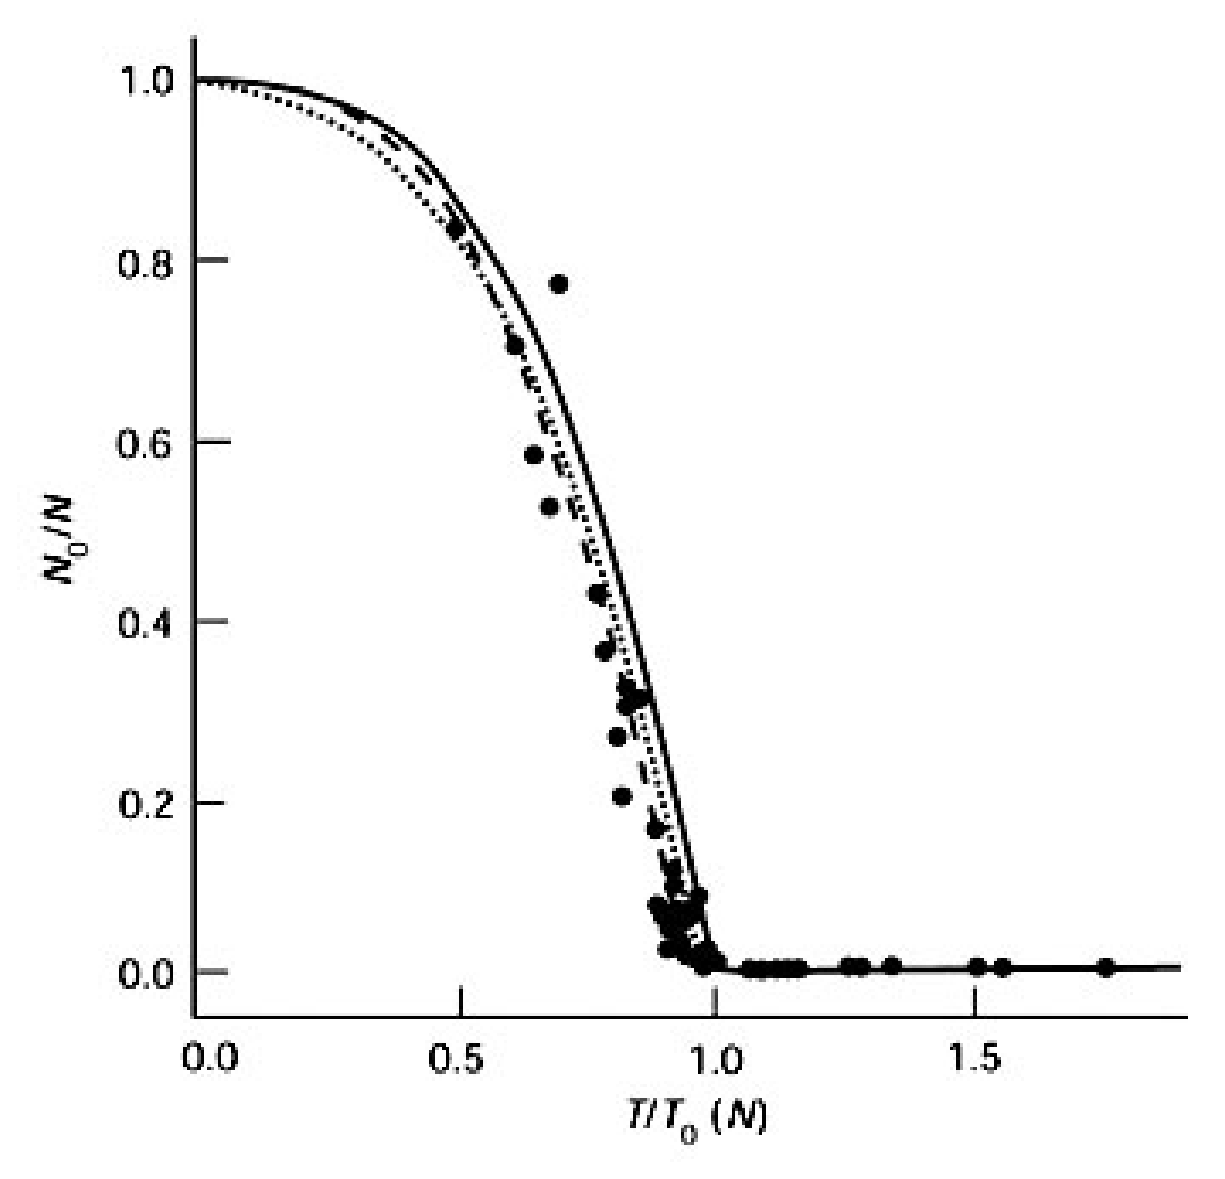
\includegraphics[clip,width=6cm]{IdenticalParticles/31-4.ps}
\caption{发生玻色-爱因斯坦凝聚的粒子百分比$N_0 / N$随温度$T_c / T$变化的关系(实验曲线)}
\end{center}
\end{figure}


\subsection*{阅读与思考}


\begin{itemize}

    \item 查阅文献,写关于``玻色-爱因斯坦凝聚''的读书报告。

   \end{itemize}
